\documentclass[aspectratio=169]{beamer}
\usepackage{fontspec}
\setsansfont{NotoSans}[Path=../fonts/,Extension=.ttf,UprightFont=*-Regular,BoldFont=*-Bold,ItalicFont=*-Italic]
\usepackage[russian]{babel}
\usepackage{graphicx,amsmath}
\setbeamertemplate{navigation symbols}{}
\setbeamertemplate{footline}{}
\setbeamercolor{frametitle}{fg=black,bg=white}
\setbeamercolor{normal text}{fg=black,bg=white}
\setbeamersize{text margin left=.55cm,text margin right=.55cm}
\newcommand{\BaseAcc}{80,63}
\newcommand{\CharAcc}{91,93}
\newcommand{\BaseCER}{19,10}
\newcommand{\CharCER}{12,67}
\newcommand{\CharGain}{11,31}
\newcommand{\CharRel}{33,66}
\newcommand{\KenAcc}{93,47}
\newcommand{\KenCER}{11,89}
\newcommand{\KenGain}{12,84}
\newcommand{\KenRel}{37,75}
\newcommand{\KenOverChar}{0,78}

\begin{document}
\begin{frame}{Быстрый языковой prior улучшает ввод в спеллере}
\vspace{-.2cm}
{\scriptsize М. А. Барабанщиков \hfill Руководитель: А. И. Майсурадзе}\par
\vspace{.1cm}
{\footnotesize \textbf{Спеллер} выбирает буквы экранной клавиатуры по реакции на стимулы.\newline
\textbf{Меняем только источник:} вероятность следующей буквы по предыдущему тексту.}
\begin{center}
\vspace{-.08cm}
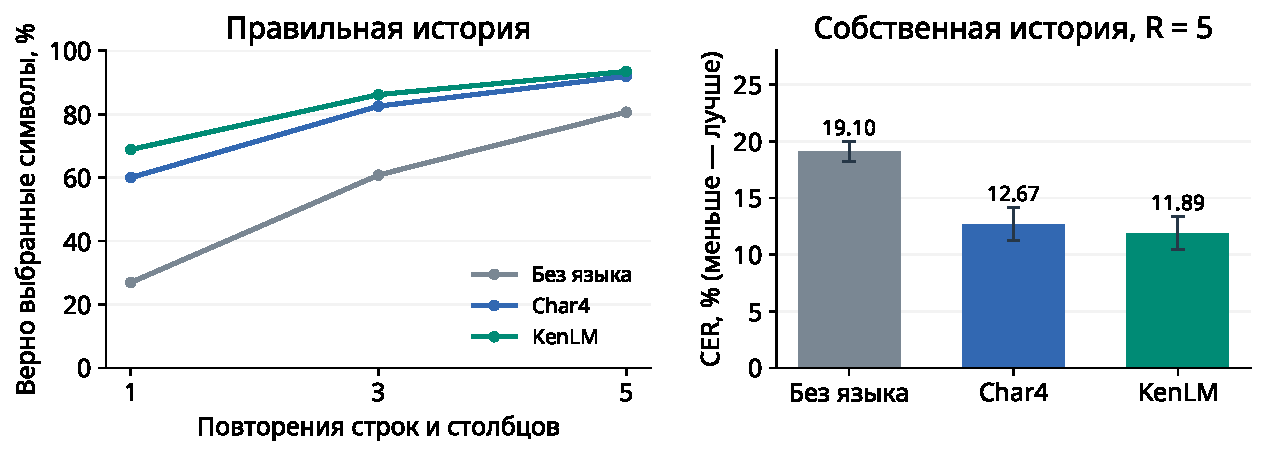
\includegraphics[width=\linewidth,height=4.1cm,keepaspectratio]{../paper/figures/native_main.pdf}
\end{center}
\vspace{-.2cm}
{\small\textbf{KenLM: CER \BaseCER\% $\rightarrow$ \KenCER\% --- на \KenRel\% меньше ошибок.}}\par
\vspace{.1cm}
{\scriptsize $q(c)\propto p_M(c\mid h)\,P(E\mid c)$; $h$ --- набранный текст, $E$ --- наблюдения.\newline
40 новых фраз $\times$ 5 seed $\times$ 3 режима = 600 сессий; физиология эмулирована.\newline
CER --- число правок / длина эталона. Посткоррекция выключена.}
\end{frame}
\end{document}
